\documentclass[11pt,letterpaper]{article}
\usepackage[lmargin=1in,rmargin=1in,tmargin=1in,bmargin=1in]{geometry}
\usepackage{../style/homework}
\usepackage{../style/commands}
\setbool{quotetype}{true} % True: Side; False: Under
\setbool{hideans}{false} % Student: True; Instructor: False

% -------------------
% Content
% -------------------
\begin{document}

\homework{6: Due 10/02}{Pitter patter, let's get at'er.}{Wayne, Letterkenny}

% Problem 1
\problem{10} For each of the following, describe whether the given dependent variable is a function of the independent variable:
	\begin{enumerate}[(a)]
	\item Independent: the number of days since you purchased your car. \par 
		Dependent: the milage for your car. 
	\item Independent: the number of people in a specific room at noon. \par 
		Dependent: the day of the week.
	\item Independent: the day of the year. \par
		Dependent: the sunrise time. 
	\item Independent: your laptop battery percentage. \par
		Dependent: the time remaining until your laptop runs out of power. 
	\end{enumerate} \pspace

\sol 
\begin{enumerate}[(a)]
\item One's car milage is a function of the number of days since they purchased the car. Given a number of days since you purchased it, there can only be one possible milage for the car. \pspace

\item The day of the week is not a function of the number of people in a room at noon. There can be the same number of people in a room at noon on many different days. For example, if one works during the day, there is likely no one in any room of the house at noon from Monday to Friday. But then given that there are no people in some room at noon, one cannot determine if the day of the week is Monday, Tuesday, Wednesday, etc. \pspace

\item The sunrise time is a function of the day of the year. Given any day of there year, there is only one possible sunrise time. \pspace

\item The time remaining until your laptop runs out of power is not a function of your laptop battery percentage. For instance, each time you fully charge the computer, the battery percentage is 100\%. However, each time you use the laptop starting a full charge, the battery may last different amount of time until running out of power based on usage, temperature, etc. 
\end{enumerate}



\newpage



% Problem 2
\problem{10} Consider the relation plotted below:
	\[
	\fbox{
	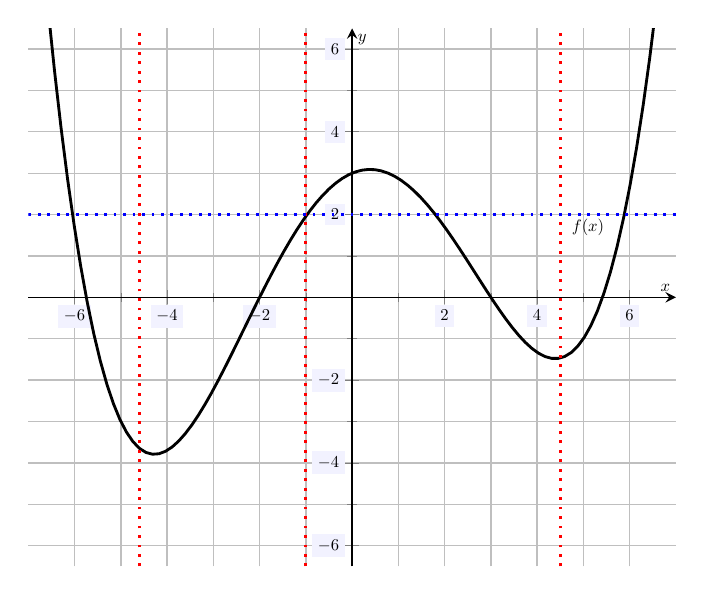
\begin{tikzpicture}[scale=1.2,every node/.style={scale=0.5}]
	\begin{axis}[
	grid=both,
	axis lines=middle,
	ticklabel style={fill=blue!5!white},
	xmin= -7, xmax=7,
	ymin= -6.5, ymax=6.5,
	xtick={-6,-4,-2,0,2,4,6},
	ytick={-6,-4,-2,0,2,4,6},
	minor tick = {-5,-3,...,5},
	xlabel=\(x\),ylabel=\(y\),
	]
	\addplot[domain=-7:7, samples=100,line width=0.03cm] (x,3 + 0.467857*x - 0.601786*x^2 - 0.0107143*x^3 + 0.0160714*x^4);
	\node at (5.1,1.7) {$f(x)$};
	
	\draw[line width=0.03cm,dotted,red] (-4.6,-6.5) -- (-4.6,6.5);
	\draw[line width=0.03cm,dotted,red] (-1,-6.5) -- (-1,6.5);
	\draw[line width=0.03cm,dotted,red] (4.5,-6.5) -- (4.5,6.5);
	
	\draw[line width=0.03cm,dotted,blue] (-7,2) -- (7,2);
	\end{axis}
	\end{tikzpicture}
	}
	\]

\begin{enumerate}[(a)]
\item Is the relation, $f(x)$, plotted above a function? Explain. 
\item Find the $y$-intercept.
\item Find the $x$-intercepts. 
\item Find the value of $f(6)$.
\item Find any $x$-values for which $f(x)= 2$.  
\end{enumerate} \pspace

\sol 
\begin{enumerate}[(a)]
\item The relation, $f(x)$, plotted above passes the Vertical Line Test; that is, every vertical line intersects the relation, $f(x)$, at most once. [See some sample vertical lines in red on the graph above.] Therefore, $f(x)$ is a function. \pspace

\item The $y$-intercept is the point (if any) where the curve intersects the $y$-axis. Examining the graph, we see that the $y$-intercept is $y= 3$, i.e. the point $(0, 3)$. 

\item The $x$-intercepts are the points (if any) where the curve intersects the $x$-axis. Examining the graph, we see that the $x$-intercepts are $x \approx -5.7469$, $-2$, $3$, and $5.41357$, i.e. the points $(-5.7469, 0)$, $(-2, 0)$, $(3, 0)$, and $(5.41357, 0)$. \pspace

\item Examining the graph, we can see the point $(6, 2.65709)$ on the graph of $f(x)$. Therefore, $f(6)= 2.65709$. 

\item Solutions to the equation $f(x)= 2$ will correspond to points where the relation $f(x)$ intersects the line $y= 2$---sketched in blue above. We see the curve intersects the line at $y= 2$ at $(-6.04388, 2)$, $(-0.972562, 2)$, $(1.79901, 2)$, and $(5.88411, 2)$. Therefore, the $x$-values for which $f(x)= 2$ are $x= -6.04388$, $-0.972562$, $1.79901$, and $5.88411$. 
\end{enumerate}



\newpage



% Problem 3
\problem{10} Define $f(x)$ to be the relation given by $f(x):= 2.7x + 14.9$.
	\begin{enumerate}[(a)]
	\item Is $f(x)$ a function? Explain.
	\item Find $f(9)$.
	\item Is there an $x_0$ so that $f(x_0)= 20$? If so, find it. If not, explain why. 
	\item Find the $y$-intercept for $f(x)$. 
	\item Find any $x$-intercepts for $f(x)$.
	\end{enumerate} \pspace

\sol 
\begin{enumerate}[(a)]
\item The relation $f(x)$ is a function. Given an input, $x$, there is only one possible output for $f(x)$---namely the one obtained by evaluating $f(x)$ at $x$. \pspace

\item We have\dots
	\[
	f(9)= 2.7(9) + 14.9= 24.3 + 14.9= 39.2 
	\] \pspace

\item If there were such an $x_0$, we would have $f(x_0)= 20$. But then\dots
	\[
	\begin{gathered}
	f(x_0)= 20 \\
	2.7x_0 + 14.9= 20 \\
	2.7x= 5.1 \\
	x\approx 1.8889
	\end{gathered}
	\]
As each step above is reversible, we know that $f(1.8889) \approx 20$. \pspace

\item The $y$-intercept for $f(x)$ is the value at which the function intercepts the $y$-axis, i.e. its value at $x= 0$. But we have $f(0)= 2.7(0) + 14.9= 0 + 14.9= 14.9$. Therefore, the $y$-intercept is $y= 14.9$, i.e. the point $(0, 14.9)$. \pspace

\item The $x$-intercepts for $f(x)$ are the value(s) (if any) where $f(x)= 0$. If $x_0$ is such a value, then we have\dots
	\[
	\begin{gathered}
	f(x_0)= 0 \\
	2.7x_0 + 14.9= 0 \\
	2.7x= -14.9 \\
	x\approx -5.51852
	\end{gathered}
	\]
As each step above is reversible, we know that $f(-5.51852) \approx 0$. Therefore, the only $x$-intercept for $f(x)$ is $x= -5.51852$, i.e. the point $(-5.51852, 0)$. 
\end{enumerate}



\newpage



% Problem 4
\problem{10} Let $f(x)$ and $g(x)$ be the functions given by the values in the table below. \par
	\begin{table}[H]
	\centering
	\begin{tabular}{r||rrrrr}
	$x$ & $-2$ & $-1$ & $0$ & $1$ & $2$ \\ \hline
	$f(x)$ & $4$ & $5$ & $-1$ & $6$ & $0$ \\
	$g(x)$ & $3$ & $-2$ & $7$ & $0$ & $-1$
	\end{tabular}
	\end{table} \par
Compute the following:
	\begin{enumerate}[(a)]
	\item $f(-2) - g(1)$ 
	\item $(f + g)(0)$
	\item $(fg)(-1)$
	\item $(f \circ g)(2)$
	\item $(g \circ f)(2)$
	\end{enumerate} \pspace

\sol 
\begin{enumerate}[(a)]
\item 
	\[
	f(-2) - g(1)= 4 - 0= 4
	\] \pspace

\item 
	\[
	(f + g)(0)= f(0) + g(0)= -1 + 7= 6
	\] \pspace
 
\item 
	\[
	(fg)(-1)= f(-1) g(-1)= 5 \cdot -2= -10
	\] \pspace
 
\item 
	\[
	(f \circ g)(2)= f \big( g(2) \big)= f(-1)= 5 
	\] \pspace
 
\item 
	\[
	(g \circ f)(2)= g \big( f(2) \big)= g(0)= 7
	\] 
\end{enumerate}


\end{document}